\chapter{Background}

\section{Radiative Heat Transfer}

    Solar thermal engines rely on thermal conductivity and radiative heat transfer for energy generation. Stefan's law was used in order to understand radiative heat transfer from sunlight to the Stirling engine. This states the relationship between power radiated by and the temperature of a material \cite{thermal}. It is thus possible to determine the power ($P$) radiated by an object:
    
    \begin{equation}
        P = \sigma eA T^{4}
        \label{stefan}
    \end{equation}
    Where $e$ is the emissivity coefficient of the object, $\sigma$ is the Stefan-Boltzmann constant ($5.6703 \cdot 10^{-8} \ W \cdot m^{-2} \cdot K^{-4}$), and A is the area of the emitting body ($m^{2}$) \cite{thermal}. Notice, for an ideal black body the emissivity coefficient is 1.
    
    The amount of radiation emitted by the sun and received by the earth is known as the solar constant $S$ ($1370 \ W \cdot m^{-2}$) \cite{thermal}. This constant is taken as an assumption since this power will vary depending on location, weather, season, and other general atmospheric factors. Therefore the solar power absorbed by an object on earth in direct sunlight is:
    
    \begin{equation}
        P_{absorbed} = SA_{i}
        \label{pwr-absorbed}
    \end{equation}
    Where $S$ is the solar constant and $A_{i}$ is the area of the object incident to the sunlight. The total power emitted from an object is given by the following:
    
    \begin{equation}
        P_{emitted} = \sigma A_{tot}T^{4}
        \label{pwr-emitted}
    \end{equation}
    Where $A_{tot}$ is the total surface area of the object and $\sigma$ and $T$ are as previously defined \cite{thermal}. These two equations, \ref{pwr-absorbed} and \ref{pwr-emitted}, can be set equal to each other in order to determine the average temperature of the object over a prolonged period of time, replacing $T$ with $T_{avg}$:
    
    \begin{equation}
        T_{avg} = \left(\frac{SA_{i}}{\sigma A_{tot}}\right)^{\frac{1}{4}}
        \label{avg-temp}
    \end{equation}
    
    This is of interest to determine the average maximum operating temperature of the piston of the Stirling engine which is incident to the sunlight. Since a lens is used to focus sunlight to the engine, the incident area $A_{i}$ is equal to the area of the Fresnel lens used in the experiment: approximately $0.056 \ m^{2}$ as measured. The total area $A_{tot}$ of the piston is approximately $0.0014 \ m^{2}$ as measured. Plugging in the necessary information to equation \ref{avg-temp} gives an average temperature of approximately 990K, or 720\degree C, assuming optimal thermal efficiency.

\section{Electricity Generation}

    Mechanical energy is converted to electricity by alternators or generators using electromagnetic induction. On the most basic level, these consist of a tightly-wound coil of wire which rotates on an axle in a magnetic field produced by permanent magnets. As the axle spins, alternating current is induced in the coil.
    
    \begin{figure}[H]
        \centering
        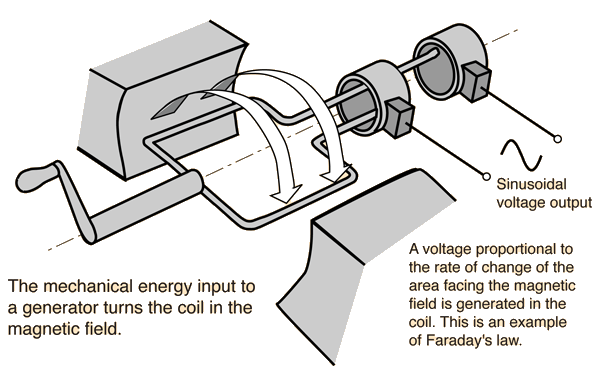
\includegraphics[width=0.75\textwidth]{diagrams/acgen}
        \caption[A.C. generator]{Alternating current generator. A coil rotates within a magnetic field to produce a sinusoidal voltage output \cite{acgen}.}
        \label{fig:acgen}
    \end{figure}
    
    Electromotive force (emf $\varepsilon$ or otherwise known as voltage $v$) can be calculated by doing the following derivation:
    
    \begin{equation}
        \Phi = \int \vec{B} \cdot d\vec{a}
        \label{eqn:flux}
    \end{equation}
    
    \[ \Phi = BA\cos\theta \]
    
    Equation \ref{eqn:flux} refers to the flux due to a magnetic field through a given surface defined by a $d\vec{a}$. $B$ is the magnitude of the magnetic field and $A$ is the area $\pi R^{2}$ enclosed by the coil where $R$ is the radius of the coil, $\theta$ is the angle between the magnetic field and the plane of the coil. In this case, $\theta = \omega t$, where $\omega$ is the angular velocity of the rotating coil within the AC generator. Therefore, by substitution:
    
    \[ \Phi = B \pi R^{2} \cos\omega t \]
    
    Which allows for the calculation of the emf $\varepsilon$:
    
    \begin{equation}
        \varepsilon = - \frac{d\Phi}{dt}
        \label{emf}
    \end{equation}
    
    \begin{equation}
        \varepsilon (t) = - \frac{d}{dt} (B \pi R^{2} \cos\omega t)
        = B \pi R^{2} \omega \sin\omega t
        \label{emft}
    \end{equation}
    
    Thus, the output of $\varepsilon (t)$ will resemble the form of Figure \ref{fig:emfsine}:
    
    \begin{figure}[H]
        \centering
        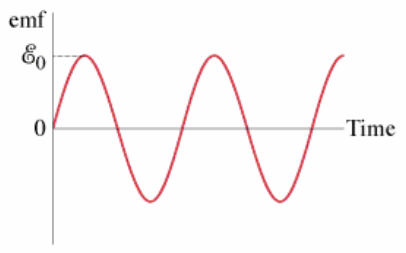
\includegraphics[width=0.5\textwidth]{diagrams/emfsine}
        \caption[EMF sine wave]{Amplitude $\varepsilon_{0} = B \pi R^{2} \omega$.}
        \label{fig:emfsine}
    \end{figure}
    
    As time progresses and the loop of wire spins in the magnetic field, the voltage output is a sinusoidal function. This is known as alternating current, or A.C..